\chapter{Introduction}
\label{sec:introduction}

\section{Motivation: Why Do Scientists Care?}
\label{sec:introduction:motivation}

\marginpar{Expand on this? Cite research tackling this problem through other means?}
The thermal properties of snow are of interest to scientists studying Arctic and
sub-Arctic climates because, during the long, cold winters in this region,
snow's thermal behavior plays a critical role in determining the net energy
balance between Earth's surface and the atmosphere. After all, any heat transfer
occurring between the Earth and the atmosphere over snow-covered ground must go
through the snow first (Figure \ref{fig:climate}). In fact, the snow
itself may store and release energy over time.

\begin{figure}[h]
\centering
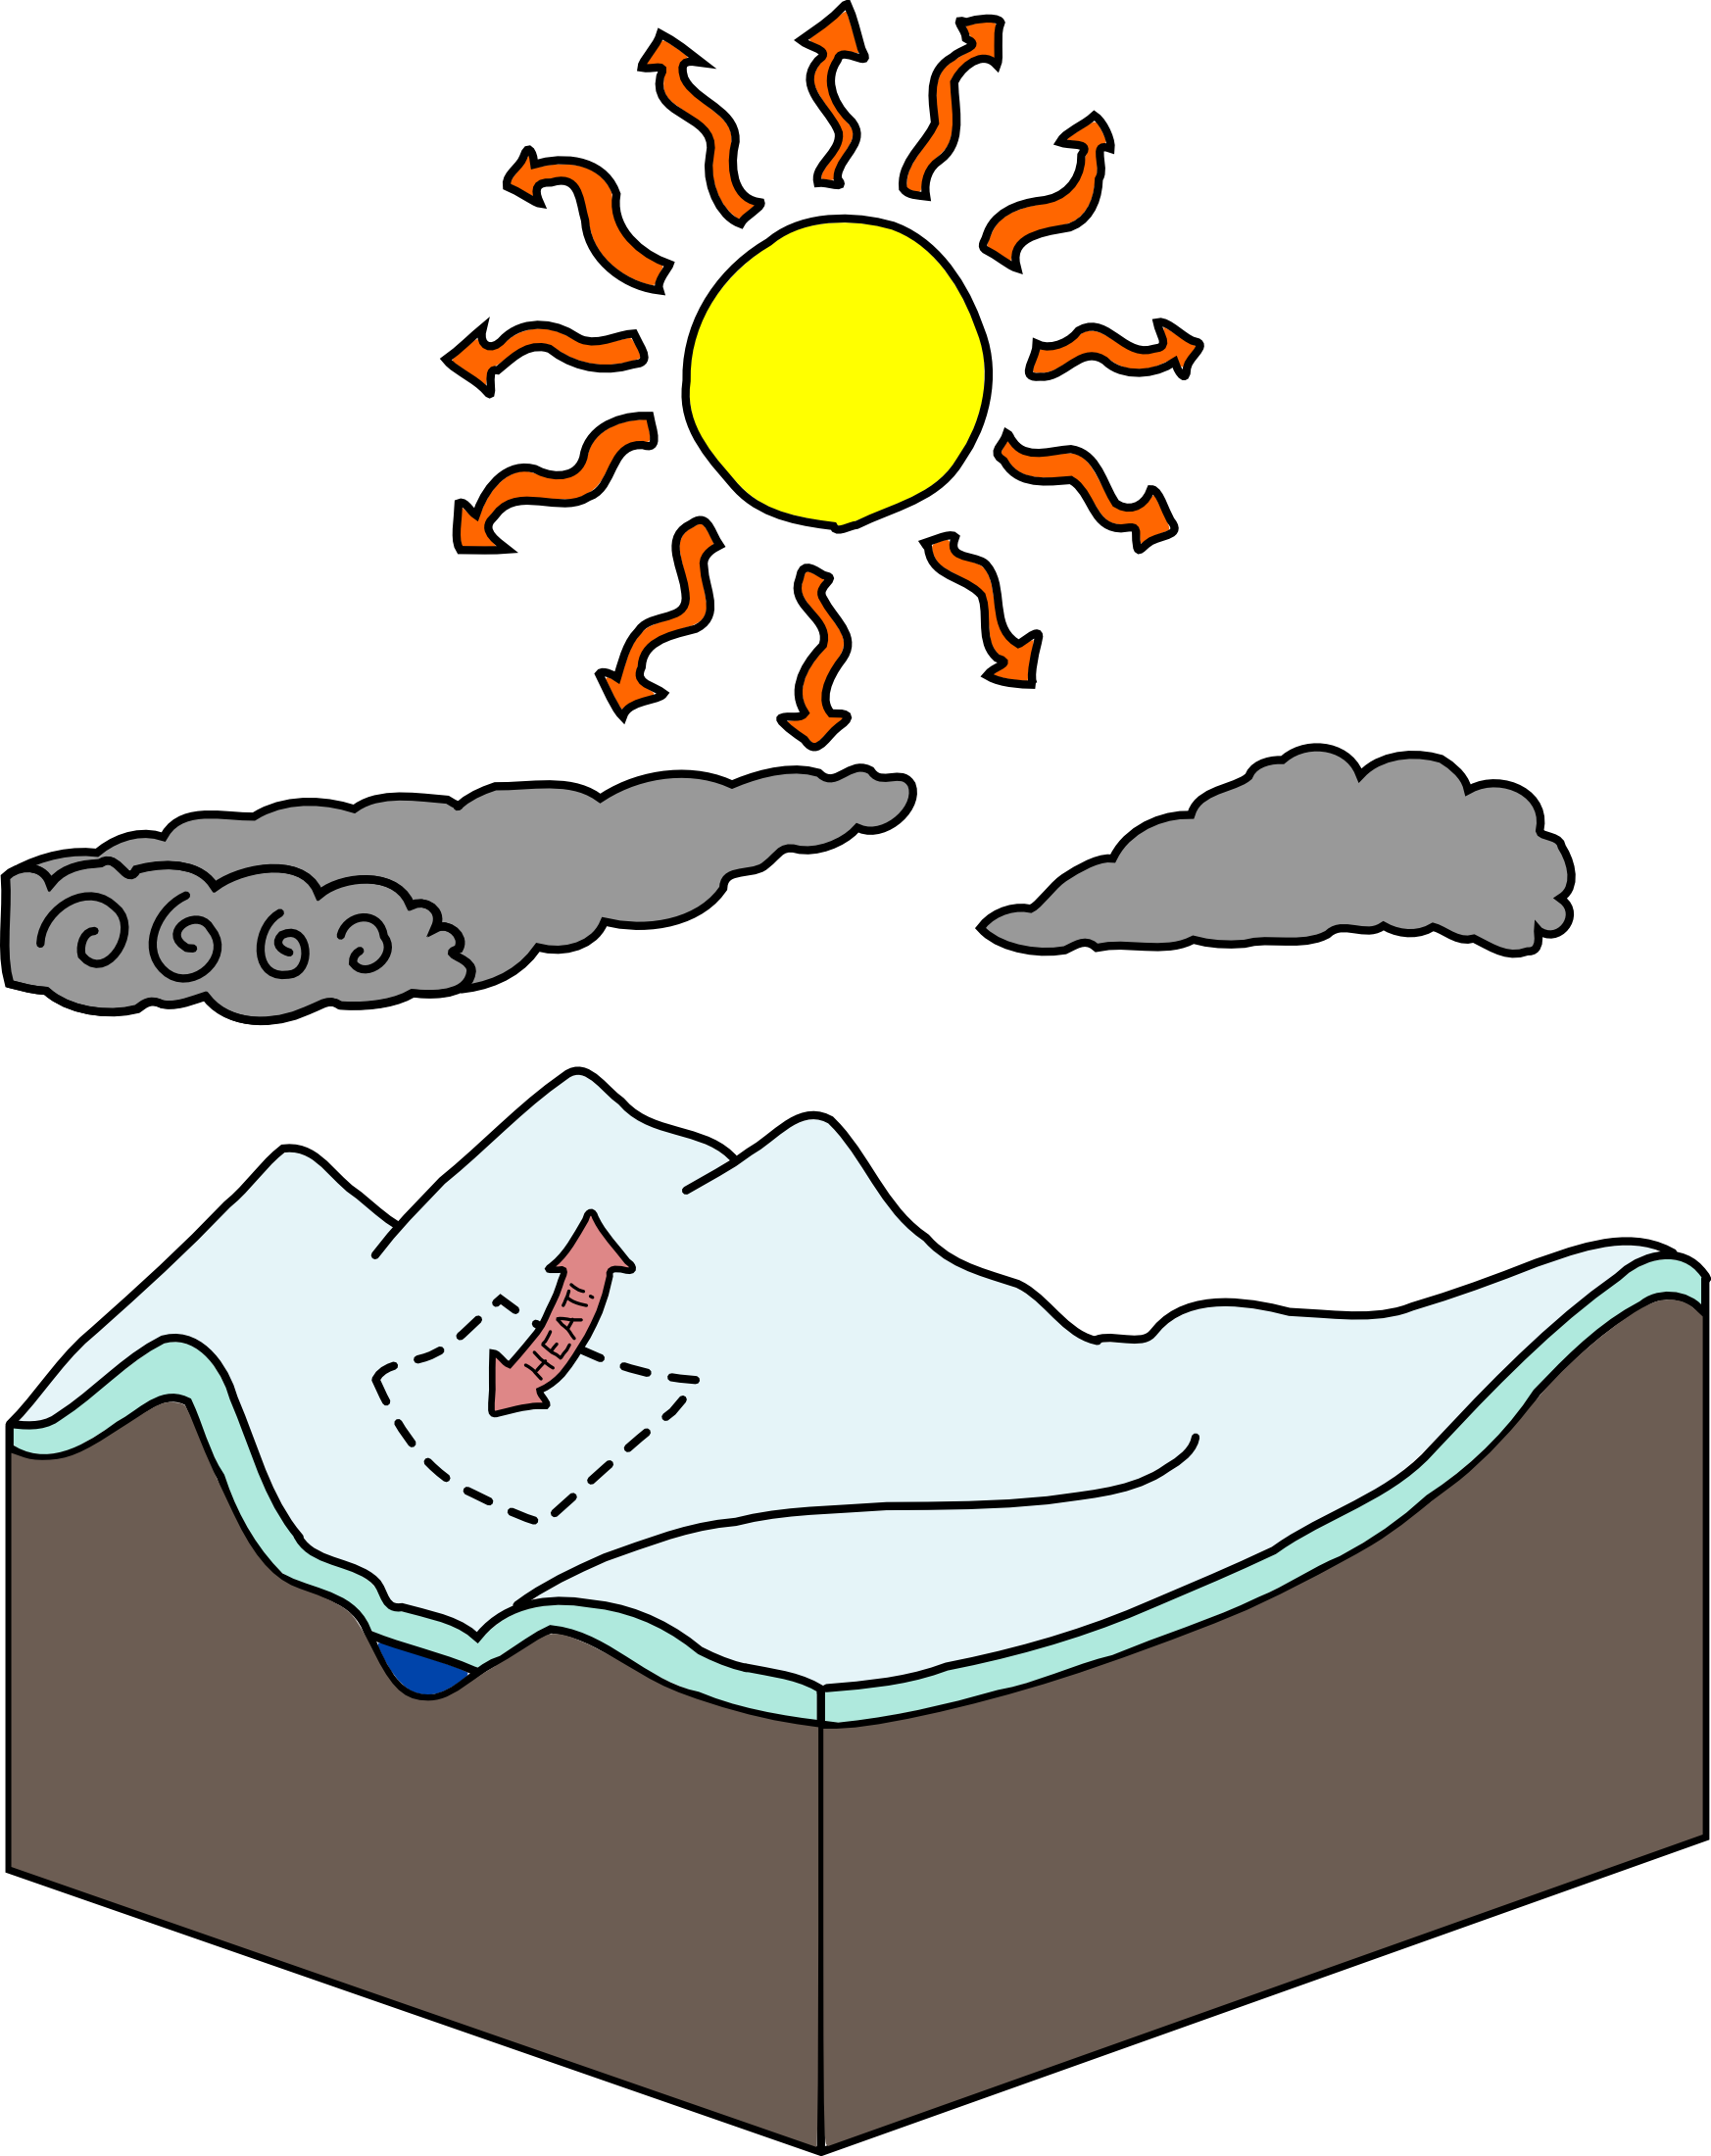
\includegraphics[width=0.4\textwidth]{fig/climate.png}
\label{fig:climate}
\caption{Arctic and Sub-Arctic climate is affected largely by heat transfer
between the atmosphere and the ground. Snowpack adds thermal resistance
transfer, affecting this heat transfer.}
\end{figure}

This energy transfer is critical in accurate climate models for these cold
regions, therefore the effective thermal conductivity of the snow is a very
important factor for these models.

\section{Needle Probes: Basic Principles}
\label{sec:introduction:needles}

A more typical technique for measuring thermal conductivity, especially in the
context of engineering materials such as building insulation, is the guarded
hot plate. For this technique, a constant temperature gradient is induced across
the material, and heat flux over the material is measured.  By Fourier's Law,
\(k = \frac{\dot{q}}{A\Delta T}\), where \(\dot{q}\) is the heat flux, \(A\) is
the cross-sectional area of the sample, and \(\Delta T\) is the temperature
difference across the sample. This technique works great in many cases. However, it is difficult to take
guarded hot plate measurements of snow because it changes structure immediately
after any physical interaction.

Another technique used for porous materials, such as soils and snow, is the
needle probe method. A needle probe consists of a long, thin needle with heating
wire running along its interior, and a temperature sensor in the center. This
configuration approximates an infinite line of constant-flux heat source
(Figure \ref{fig:needle_xsect}).

\marginpar{Don't have this image in fig/ :(}
\begin{figure}[h]
\centering
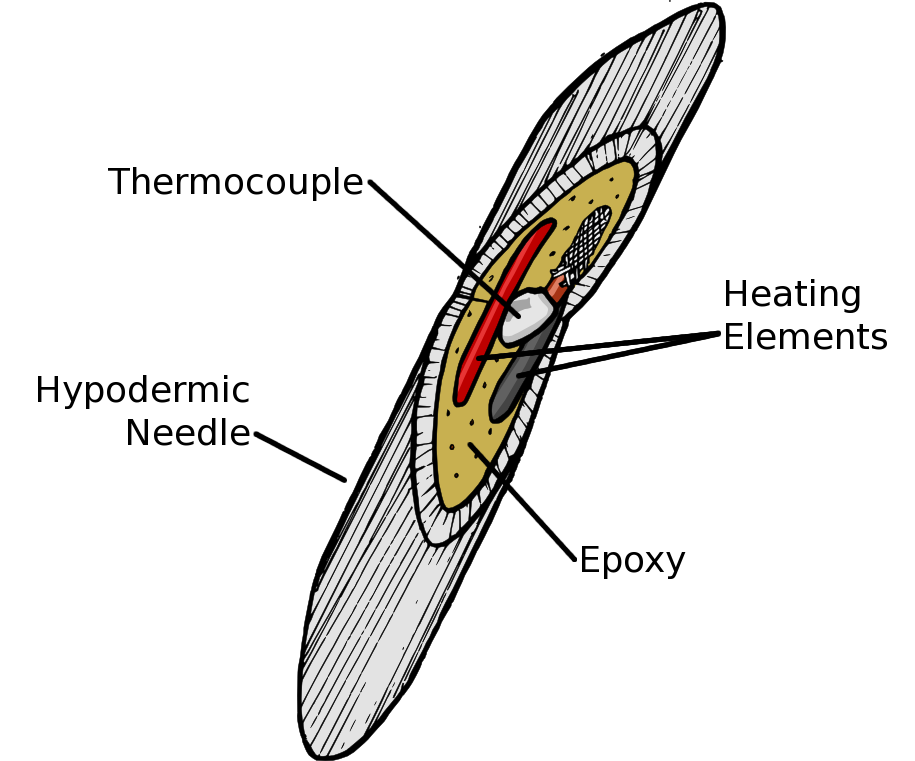
\includegraphics[width=0.2\textwidth]{fig/needle_xsect.png}
\label{fig:needle_xsect}
\caption{An illustration of a needle probe in cross-section. Note that the heat
trace in many needle probes, including the one used in experiments for this
research, actually wraps around an inner core instead of running axially through
the needle.}
\end{figure}

This needle is inserted into the material whose thermal conductivity is being
measured, and a constant voltage is applied to the needle's heating element.
This causes a constant heat flux along the needle, and, knowing the resistance
of the heat trace, this heat flux may be calculated. This causes the material's
temperature near the needle to rise (Figure \ref{fig:heating_curve}. After some
given amount of time, the heating element is turned off, and the temperature
around the needle begins to fall back towards ambient (Figure \ref{fig:cooling_curve}).
The temperature data measured over time for these two periods are called the
heating curve and cooling curve, respectively.  Based on the slopes of these
curves as a function of \(\ln(t)\) and approximate analytical solutions for
these situations, effective thermal conductivity may be calculated.

The specifics of these solutions are explored more thoroughly in chapter
\ref{sec:analytical-np}.

\section{Snow Metamorphic Principles}
\label{sec:introduction:metamorphic}
